%% bare_conf.tex
%% V1.3
%% 2007/01/11
%% by Michael Shell
%% See:
%% http://www.michaelshell.org/
%% for current contact information.
%%
%% This is a skeleton file demonstrating the use of IEEEtran.cls
%% (requires IEEEtran.cls version 1.7 or later) with an IEEE conference paper.
%%
%% Support sites:
%% http://www.michaelshell.org/tex/ieeetran/
%% http://www.ctan.org/tex-archive/macros/latex/contrib/IEEEtran/
%% and
%% http://www.ieee.org/

%%*************************************************************************
%% Legal Notice:
%% This code is offered as-is without any warranty either expressed or
%% implied; without even the implied warranty of MERCHANTABILITY or
%% FITNESS FOR A PARTICULAR PURPOSE!
%% User assumes all risk.
%% In no event shall IEEE or any contributor to this code be liable for
%% any damages or losses, including, but not limited to, incidental,
%% consequential, or any other damages, resulting from the use or misuse
%% of any information contained here.
%%
%% All comments are the opinions of their respective authors and are not
%% necessarily endorsed by the IEEE.
%%
%% This work is distributed under the LaTeX Project Public License (LPPL)
%% ( http://www.latex-project.org/ ) version 1.3, and may be freely used,
%% distributed and modified. A copy of the LPPL, version 1.3, is included
%% in the base LaTeX documentation of all distributions of LaTeX released
%% 2003/12/01 or later.
%% Retain all contribution notices and credits.
%% ** Modified files should be clearly indicated as such, including  **
%% ** renaming them and changing author support contact information. **
%%
%% File list of work: IEEEtran.cls, IEEEtran_HOWTO.pdf, bare_adv.tex,
%%                    bare_conf.tex, bare_jrnl.tex, bare_jrnl_compsoc.tex
%%*************************************************************************

% *** Authors should verify (and, if needed, correct) their LaTeX system  ***
% *** with the testflow diagnostic prior to trusting their LaTeX platform ***
% *** with production work. IEEE's font choices can trigger bugs that do  ***
% *** not appear when using other class files.                            ***
% The testflow support page is at:
% http://www.michaelshell.org/tex/testflow/



% Note that the a4paper option is mainly intended so that authors in
% countries using A4 can easily print to A4 and see how their papers will
% look in print - the typesetting of the document will not typically be
% affected with changes in paper size (but the bottom and side margins will).
% Use the testflow package mentioned above to verify correct handling of
% both paper sizes by the user's LaTeX system.
%
% Also note that the "draftcls" or "draftclsnofoot", not "draft", option
% should be used if it is desired that the figures are to be displayed in
% draft mode.
%
\newcommand{\CLASSINPUTinnersidemargin}{1in}
\documentclass[10pt, conference, letterpaper]{IEEEtran}
% Add the compsoc option for Computer Society conferences.
%
% If IEEEtran.cls has not been installed into the LaTeX system files,
% manually specify the path to it like:
% \documentclass[conference]{../sty/IEEEtran}


\usepackage{caption2}


% Some very useful LaTeX packages include:
% (uncomment the ones you want to load)


% *** MISC UTILITY PACKAGES ***
%
%\usepackage{ifpdf}
% Heiko Oberdiek's ifpdf.sty is very useful if you need conditional
% compilation based on whether the output is pdf or dvi.
% usage:
% \ifpdf
%   % pdf code
% \else
%   % dvi code
% \fi
% The latest version of ifpdf.sty can be obtained from:
% http://www.ctan.org/tex-archive/macros/latex/contrib/oberdiek/
% Also, note that IEEEtran.cls V1.7 and later provides a builtin
% \ifCLASSINFOpdf conditional that works the same way.
% When switching from latex to pdflatex and vice-versa, the compiler may
% have to be run twice to clear warning/error messages.






% *** CITATION PACKAGES ***
%
%\usepackage{cite}
% cite.sty was written by Donald Arseneau
% V1.6 and later of IEEEtran pre-defines the format of the cite.sty package
% \cite{} output to follow that of IEEE. Loading the cite package will
% result in citation numbers being automatically sorted and properly
% "compressed/ranged". e.g., [1], [9], [2], [7], [5], [6] without using
% cite.sty will become [1], [2], [5]--[7], [9] using cite.sty. cite.sty's
% \cite will automatically add leading space, if needed. Use cite.sty's
% noadjust option (cite.sty V3.8 and later) if you want to turn this off.
% cite.sty is already installed on most LaTeX systems. Be sure and use
% version 4.0 (2003-05-27) and later if using hyperref.sty. cite.sty does
% not currently provide for hyperlinked citations.
% The latest version can be obtained at:
% http://www.ctan.org/tex-archive/macros/latex/contrib/cite/
% The documentation is contained in the cite.sty file itself.





\usepackage{cite}
% *** GRAPHICS RELATED PACKAGES ***
%
\ifCLASSINFOpdf
  % \usepackage[pdftex]{graphicx}
  % declare the path(s) where your graphic files are
  % \graphicspath{{../pdf/}{../jpeg/}}
  % and their extensions so you won't have to specify these with
  % every instance of \includegraphics
  % \DeclareGraphicsExtensions{.pdf,.jpeg,.png}
\else
  % or other class option (dvipsone, dvipdf, if not using dvips). graphicx
  % will default to the driver specified in the system graphics.cfg if no
  % driver is specified.
   \usepackage[dvips]{graphicx}
  % declare the path(s) where your graphic files are
   \graphicspath{{../eps/}}
  % and their extensions so you won't have to specify these with
  % every instance of \includegraphics
   \DeclareGraphicsExtensions{.eps}
\fi
% graphicx was written by David Carlisle and Sebastian Rahtz. It is
% required if you want graphics, photos, etc. graphicx.sty is already
% installed on most LaTeX systems. The latest version and documentation can
% be obtained at:
% http://www.ctan.org/tex-archive/macros/latex/required/graphics/
% Another good source of documentation is "Using Imported Graphics in
% LaTeX2e" by Keith Reckdahl which can be found as epslatex.ps or
% epslatex.pdf at: http://www.ctan.org/tex-archive/info/
%
% latex, and pdflatex in dvi mode, support graphics in encapsulated
% postscript (.eps) format. pdflatex in pdf mode supports graphics
% in .pdf, .jpeg, .png and .mps (metapost) formats. Users should ensure
% that all non-photo figures use a vector format (.eps, .pdf, .mps) and
% not a bitmapped formats (.jpeg, .png). IEEE frowns on bitmapped formats
% which can result in "jaggedy"/blurry rendering of lines and letters as
% well as large increases in file sizes.
%
% You can find documentation about the pdfTeX application at:
% http://www.tug.org/applications/pdftex





% *** MATH PACKAGES ***
%
%\usepackage[cmex10]{amsmath}
% A popular package from the American Mathematical Society that provides
% many useful and powerful commands for dealing with mathematics. If using
% it, be sure to load this package with the cmex10 option to ensure that
% only type 1 fonts will utilized at all point sizes. Without this option,
% it is possible that some math symbols, particularly those within
% footnotes, will be rendered in bitmap form which will result in a
% document that can not be IEEE Xplore compliant!
%
% Also, note that the amsmath package sets \interdisplaylinepenalty to 10000
% thus preventing page breaks from occurring within multiline equations. Use:
%\interdisplaylinepenalty=2500
% after loading amsmath to restore such page breaks as IEEEtran.cls normally
% does. amsmath.sty is already installed on most LaTeX systems. The latest
% version and documentation can be obtained at:
% http://www.ctan.org/tex-archive/macros/latex/required/amslatex/math/





% *** SPECIALIZED LIST PACKAGES ***
%
%\usepackage{algorithmic}
% algorithmic.sty was written by Peter Williams and Rogerio Brito.
% This package provides an algorithmic environment fo describing algorithms.
% You can use the algorithmic environment in-text or within a figure
% environment to provide for a floating algorithm. Do NOT use the algorithm
% floating environment provided by algorithm.sty (by the same authors) or
% algorithm2e.sty (by Christophe Fiorio) as IEEE does not use dedicated
% algorithm float types and packages that provide these will not provide
% correct IEEE style captions. The latest version and documentation of
% algorithmic.sty can be obtained at:
% http://www.ctan.org/tex-archive/macros/latex/contrib/algorithms/
% There is also a support site at:
% http://algorithms.berlios.de/index.html
% Also of interest may be the (relatively newer and more customizable)
% algorithmicx.sty package by Szasz Janos:
% http://www.ctan.org/tex-archive/macros/latex/contrib/algorithmicx/




% *** ALIGNMENT PACKAGES ***
%
%\usepackage{array}
% Frank Mittelbach's and David Carlisle's array.sty pFDRChes and improves
% the standard LaTeX2e array and tabular environments to provide better
% appearance and additional user controls. As the default LaTeX2e table
% generation code is lacking to the point of almost being broken with
% respect to the quality of the end results, all users are strongly
% advised to use an enhanced (at the very least that provided by array.sty)
% set of table tools. array.sty is already installed on most systems. The
% latest version and documentation can be obtained at:
% http://www.ctan.org/tex-archive/macros/latex/required/tools/


%\usepackage{mdwmath}
%\usepackage{mdwtab}
% Also highly recommended is Mark Wooding's extremely powerful MDW tools,
% especially mdwmath.sty and mdwtab.sty which are used to format equations
% and tables, respectively. The MDWtools set is already installed on most
% LaTeX systems. The lastest version and documentation is available at:
% http://www.ctan.org/tex-archive/macros/latex/contrib/mdwtools/


% IEEEtran contains the IEEEeqnarray family of commands that can be used to
% generate multiline equations as well as matrices, tables, etc., of high
% quality.


%\usepackage{eqparbox}
% Also of notable interest is Scott Pakin's eqparbox package for creating
% (automatically sized) equal width boxes - aka "natural width parboxes".
% Available at:
% http://www.ctan.org/tex-archive/macros/latex/contrib/eqparbox/



\usepackage[caption=false,font=footnotesize]{subfig}
\usepackage{url}
\usepackage{amsmath}
\usepackage{amsfonts}
\newtheorem{definition}{\noindent{\bf Definition}}
\newtheorem{lemma}{\noindent{\bf Lemma}}
\newtheorem{theorem}{\noindent{\bf Theorem}}
\newtheorem{proposition}{\noindent{\bf proposition}}
\usepackage{algorithm}              
\usepackage{algorithmic}            
\usepackage{multirow}             
\usepackage{amsmath} 
\usepackage{xcolor} 
\DeclareMathOperator*{\argmin}{argmin}     
\renewcommand{\algorithmicrequire}{\textbf{Input:}}  
\renewcommand{\algorithmicensure}{\textbf{Output:}}  % *** SUBFIGURE PACKAGES ***
%\usepackage[tight,footnotesize]{subfigure}
% subfigure.sty was written by Steven Douglas Cochran. This package makes it
% easy to put subfigures in your figures. e.g., "Figure 1a and 1b". For IEEE
% work, it is a good idea to load it with the tight package option to reduce
% the amount of white space around the subfigures. subfigure.sty is already
% installed on most LaTeX systems. The latest version and documentation can
% be obtained at:
% http://www.ctan.org/tex-archive/obsolete/macros/latex/contrib/subfigure/
% subfigure.sty has been superceeded by subfig.sty.



%\usepackage[caption=false]{caption}
%\usepackage[font=footnotesize]{subfig}
% subfig.sty, also written by Steven Douglas Cochran, is the modern
% replacement for subfigure.sty. However, subfig.sty requires and
% automatically loads Axel Sommerfeldt's caption.sty which will override
% IEEEtran.cls handling of captions and this will result in nonIEEE style
% figure/table captions. To prevent this problem, be sure and preload
% caption.sty with its "caption=false" package option. This is will preserve
% IEEEtran.cls handing of captions. Version 1.3 (2005/06/28) and later
% (recommended due to many improvements over 1.2) of subfig.sty supports
% the caption=false option directly:
%\usepackage[caption=false,font=footnotesize]{subfig}
%
% The latest version and documentation can be obtained at:
% http://www.ctan.org/tex-archive/macros/latex/contrib/subfig/
% The latest version and documentation of caption.sty can be obtained at:
% http://www.ctan.org/tex-archive/macros/latex/contrib/caption/




% *** FLOAT PACKAGES ***
%
%\usepackage{fixltx2e}
% fixltx2e, the successor to the earlier fix2col.sty, was written by
% Frank Mittelbach and David Carlisle. This package corrects a few problems
% in the LaTeX2e kernel, the most notable of which is that in current
% LaTeX2e releases, the ordering of single and double column floats is not
% guaranteed to be preserved. Thus, an unpFDRChed LaTeX2e can allow a
% single column figure to be placed prior to an earlier double column
% figure. The latest version and documentation can be found at:
% http://www.ctan.org/tex-archive/macros/latex/base/



%\usepackage{stfloats}
% stfloats.sty was written by Sigitas Tolusis. This package gives LaTeX2e
% the ability to do double column floats at the bottom of the page as well
% as the top. (e.g., "\begin{figure*}[!b]" is not normally possible in
% LaTeX2e). It also provides a command:
%\fnbelowfloat
% to enable the placement of footnotes below bottom floats (the standard
% LaTeX2e kernel puts them above bottom floats). This is an invasive package
% which rewrites many portions of the LaTeX2e float routines. It may not work
% with other packages that modify the LaTeX2e float routines. The latest
% version and documentation can be obtained at:
% http://www.ctan.org/tex-archive/macros/latex/contrib/sttools/
% Documentation is contained in the stfloats.sty comments as well as in the
% presfull.pdf file. Do not use the stfloats baselinefloat ability as IEEE
% does not allow \baselineskip to stretch. Authors submitting work to the
% IEEE should note that IEEE rarely uses double column equations and
% that authors should try to avoid such use. Do not be tempted to use the
% cuted.sty or midfloat.sty packages (also by Sigitas Tolusis) as IEEE does
% not format its papers in such ways.





% *** PDF, URL AND HYPERLINK PACKAGES ***
%
%\usepackage{url}
% url.sty was written by Donald Arseneau. It provides better support for
% handling and breaking URLs. url.sty is already installed on most LaTeX
% systems. The latest version can be obtained at:
% http://www.ctan.org/tex-archive/macros/latex/contrib/misc/
% Read the url.sty source comments for usage information. Basically,
% \url{my_url_here}.





% *** Do not adjust lengths that control margins, column widths, etc. ***
% *** Do not use packages that alter fonts (such as pslatex).         ***
% There should be no need to do such things with IEEEtran.cls V1.6 and later.
% (Unless specifically asked to do so by the journal or conference you plan
% to submit to, of course. )


% correct bad hyphenation here
\hyphenation{op-tical net-works semi-conduc-tor DCTCP long-term}
\begin{document}
\title{ FDRC -- Flow Duration Time Based Rate Control in Data Center Networks }
\author{\IEEEauthorblockN{Han Zhang\IEEEauthorrefmark{1}\IEEEauthorrefmark{3},  Xingang Shi\IEEEauthorrefmark{2}\IEEEauthorrefmark{3}, Xia Yin\IEEEauthorrefmark{1}\IEEEauthorrefmark{3}, Zhiliang Wang\IEEEauthorrefmark{2}\IEEEauthorrefmark{3},YingYa Guo\IEEEauthorrefmark{1}\IEEEauthorrefmark{3}}
\IEEEauthorblockA{\IEEEauthorrefmark{1}Department of Computer Science and Technology, Tsinghua University\\
\IEEEauthorrefmark{2}Institute for Network Sciences and Cyberspace, Tsinghua University\\
\IEEEauthorrefmark{3}Tsinghua National Laboratory for Information Science and Technology (TNLIST)\\
Beijing, P.R. China\\
Email:\{zhanghan, wzl, yxia,guoyingya\}@csnet1.cs.tsinghua.edu.cn, \{shixg\}@cernet.edu.cn
}
}

% make the title area
\maketitle


\begin{abstract}

Data Center is now becoming an important facility for many applications (e.g, web search and retail).
As TCP can't meet applications' demands for latency and throughput, 
many tcp-based protocols (e.g, DCTCP, D2TCP, L2DCT) have been proposed.
Among them, protocols such as D2TCP incorporate explicit deadline into congestion window adjustment procedure to guarantee flows' latency and 
protocols such as L2DCT consider flow size when computing congestion window adjustment factor to guarantee the throughput of short flows. 
These two methods work well at some scenery but they have some deficiencies on two aspects.
Firstly, we find that they can only reduce the percentage of flows missing deadline or reduce flow completion time, 
but can not meet both the goals simultaneously.
Secondly, most of these methods need the user to know flow information (e.g, deadline, flow size),
which may be hard to know exact value beforehand. 
In this paper, we advocate to use flow duration time into congestion window adjustment procedure.
Based on this, we propose FDRC--Flow Duration Time based Rate Control algorithm.
We find that without knowing flow information beforehand,
FDRC can achieve the goal of reducing the percentage of flows missing deadline
and cutting average flow completion time simultaneously. 
We theoretically analyze FDRC's behavior and implement FDRC into ns-2 as well as linux kernel.  
Our experiments show that FDRC performs better than D2TCP and L2DCT at nearly all the scenarios. 
On average, it performs 30\% better than the state-of-art deadline-aware congestion control protocol D2TCP and 
10\% better than the state-of-art flowsize-aware protocol L2DCT.
\end{abstract}


\section{Introduction} \label{Introduction}
Nowadays, more and more latency-sensitive applications (e.g, web search, retail) are deployed in data center networks.  
Data center networks (DCNs) require
high throughput, low latency and high burst tolerance\cite{guo2014traffic}\cite{LPD}\cite{zhang2015towards}. Recently, among these characters, 
latency attracts more attention, as it affects user experience in these applications and thus revenue.
Indeed, every additional 100ms can cause 1\% loss of revenue \cite{DCTCP}.

In particular, traffic in data center is mixture of  
long-live background traffic, delay-sensitive traffic and bandwidth-sensitive traffic, the traditional transport mechanism TCP falls short on two sides.
Firstly, TCP can cause buffers overflow and this will affect user experience.
Secondly, window will cut by half when congestion happens and this causes 
link utilization low.  Due to the pitfalls of TCP, DCTCP\cite{DCTCP} is proposed. DCTCP uses ECN marking mechanism\cite{DCTCP} which is supported by most modern switch to give feedback to senders, so that
senders can adjust its congestion window according to congestion degree. 
DCTCP keeps switch's queue shallow and maintain link utilization high.
However, DCTCP is deadline-agnostic and it treats all flows fair and many delay-sensitive flows will miss their time constraints \cite{D3}\cite{D2TCP}.
Then two types of methods are proposed to make up the deficiencies:

\emph{Set explicit deadline to flows}. 
D3 \cite{D3}, D2TCP \cite{D2TCP} and LPD \cite{LPD} allow users to set explicit deadline to flows from
user space, so that congestion window can adapt to fit the time constraints. 
As a result, those emergency flows will get relatively larger bandwidth than the lax 
ones and this can help more flows finish before time constraints.

\emph{Set high priority to short flows}.  
In DCNs, time-constraint flows are always short \cite{PDQ}, so another class methods
such as PDQ \cite{PDQ}, L2DCT \cite{L2DCT} and pFabric \cite{pFabric} try to set short flows high priority. 
They try to realize SJF (shortest job first) schema, 
which proves to be optimal for reducing average flow completion time in single bottleneck link scenery, 
so that more short urgent flows can finish before time constraints.


We conclude that both methods try to set higher priority to urgent flows to let more flows finish before time constraints. 
The difference between them is that 
the first kind of methods set priority according to users' expected latency the second kind set priority according to flow size.
Both methods need the users to know flow information beforehand. 
That means, if we use the first class of protocols, we should know flow time constraints in advance and 
if we use the second class, flow size is needed beforehand.
Besides, traffic in data center is mixture of delay-sensitive flow, bandwidth-sensitive flow and long-live background flow, the first class of methods
just meet the requirements of delay-sensitive flow and the second class of methods just tries to reduce average flow completion time.
Neither of the methods can meet the demands simultaneously.



Because of the flaws, we advocate flow's priority can be set according to duration time from flow starting. 
Flows have the highest priority when they begin to transfer and their priority descends as time goes on.
We think this a good choice, because
on one hand, we do not need to know flow information (flow size or deadline) beforehand;
on the other hand, by setting high priority to those short duration ones,  
the latency-constraint flows and the small flows will get more bandwidth on average,
so that the demands of reducing the percentage of flows missing time constraints and reducing average flow completion time can be met.
Based on this, we propose FDRC-Flow Duration Time Based Rate Control algorithm.
We implement FDRC into ns-2  \cite{ns2} and linux kernel 3.2.61.
Our experiment results demonstrate FDRC improves about 30\% over D2TCP and 2X over DCTCP. 
Thus the contribution we make in this paper:


\begin{itemize}[\IEEEsetlabelwidth{Z}]
\item A data center transport protocol FDRC that helps more flows to meet deadline and helps to reduce average flow completion time.
\item Design and analyze congestion control mechanism-- FDRC which can reduce the percentage of flows missing deadline without setting explicit information to flows in advance.
\item Extensive evaluation of FDRC in ns-2, then compare FDRC with DCTCP, D2TCP, L2DCT, LPD and pFabric.
\item Evaluate FDRC into linux kernel and construct small data center testbed to test the performance of FDRC.
\end{itemize}




The rest of our paper is organized as follows. 
We first introduce some necessary background and related work in Section \ref{Background}. 
In Section \ref{protocol}, we propose FDRC and the we analyze it. 
Then we evaluate FDRC in Section \ref{evaluation} both by simulation and in real testbed. 
At last , we concludes the paper at Section \ref{conclusion}.




\section{Background and related work} \label{Background}

The ever-increasingly used data center networks, although often have ultra high bandwidth and low latency links, still face frequent network congestions.
As many applications (i.e. OLDI, web search) call for low latency and the traditional transport TCP can cause a large percentage of flows missing time constraints
, so many new schedule and transport protocols are raised to be suited to these small urgent flows.



To keep switch buffer shallow, DCTCP \cite{DCTCP} uses ECN marking mechanism.  
When packets arrive, if queue size is larger than threshold K, packets will be marked. Senders
then compute$\alpha$ which reflects congestion degree.  Then congestion window will be computed as
$w=w*(1-\alpha/2)$. DCTCP reduces congestion window according to link congestion degree. 
With the help of ECN marking mechanism, DCTCP  has small queue delay.
DCTCP is hardware-friendly protocol.
However, for some applications like web search, DCTCP's fair sharing is not a good choice, because flows in these applications
call for different time constraints. Fair sharing policy can cause some urgent flows miss their time constrains.




Since different flows call for different latency, D3 \cite{D3} tries to set soft deadline constrains to flows. Bandwidth is computed at the sender side
according to deadline, so urgent flows can get more bandwidth than lax ones, as a result, more flows will finish before their time constraints.
Although D3 improves much over DCTCP, it also has some drawbacks:
on one hand, it does changes to switch hardware and can not coexist with TCP; 
on the other hand, it is shown to work bad in some race conditions where far-deadline requests arrive slightly ahead of near-deadline requests due to its greedy and first-come-first-service policy \cite{D2TCP}.




Based on DCTCP, D2TCP \cite{D2TCP} sets deadline constraints to flows, so urgent flows will have smaller congestion window reduction than lax ones.
In D2TCP, flows reduce congestion window using $w=w*(1-\alpha^d)$, where $\alpha$ is the congestion level as DCTCP and $d=TC/D$ is deadline factor.
$TC$ can be understood as the time needed for flow to complete its transmitting under the deadline-agnostic manner and D is the remaining time till deadline. 
D2TCP can coexist with TCP and does not need to change switch hardware.
D2TCP's performance drops  when load becomes heavy. 

 LPD \cite{LPD} finds the defects of D2TCP and advocate congestion control function should follow the principle:
 more load, more differentiation. That means when load is heavy,  it is more necessary to differentiate flows with different deadline request.
 LPD uses the linear function $f=\alpha*t/t_{max}$. LPD can co-exist with TCP and does not need to change switch hardware. 
 

Until now, D3, D2TCP and LPD all try to set deadline to flows.
As in data center networks,  those time urgent flows are always the short ones , another class method tries to reduce average flow completion time or tail to help these ones finish before time constraints.
As at single bottleneck link, SJF is considered to be optimal, so flow size is often chosen as the parameter.




L2DCT \cite{L2DCT} bases on DCTCP and it alters both
the additive increase part as well as the multiplicative decrease part of the window computation.
L2DCT also uses gamma function as its penalty function, which is the same as D2TCP. 
In L2DCT, short flow have larger congestion window increment and smaller congestion window decrement than large flows.
As a result, average flow completion time will be reduced.



PDQ \cite{PDQ} is a schedule method. PDQ works in distributed fashion which is different from D3.
PDQ can  emulate different scheduling policies like Earliest Deadline First (EDF) or Shortest Job First (SJF).
However,  PDQ should change switch hardware and can not co-exist with TCP.

pFabric \cite{pFabric} advocates datacenter transport should decouple flow scheduling from rate control. 
For flow scheduling, it uses Shortest Remaining Processing Time (SRPT) policy and for rate control. Flows start at line rate and throttle back only under high and persistent packet loss.
Combining these two characters, pFabric achieve near-optimal performance for flow completion time. 
pFabric changes switch and can not co-exist with TCP.


PASE \cite{PASE} claims protocols (DCTCP, PDQ, pFabric, etc) are not competitors, 
they are complementary. 
PASE does not change network elements and its
performance is better than those state-of-art protocols \cite{PASE}.


We can summarize that all these protocols, no matter explicit or implicit, 
all need to set parameters (flow size, deadline, remaining flow size, remaining time,etc) or change network
hardware.
However, in data center, traffic is mixture of delay-sensitive flow, bandwidth-sensitive flow and long-live background flow, setting deadline to flows
just reducing the percentage of flows missing deadline and using flow size can only reduce the average flow completion time of flows.
Neither of the methods can meet both the demands at the same time.
What we need is to meet the requirements simultaneously and do not need the user to provide flow information beforehand.



\begin{figure*}[!htb]
\centering
\subfloat[percentage of flows missing deadline]{
\label{spine-dc-data2-1}
\includegraphics[width=0.33\textwidth]{picture/motivation/miss_deadline.eps}}
\subfloat[average flow completion time]{
\label{spine-dc-data2-5}
\includegraphics[width=0.33\textwidth]{picture/motivation/fct.eps}}
\subfloat[background traffic bandwidth]{
\label{spine-dc-data2-30}
\includegraphics[width=0.33\textwidth]{picture/motivation/bandwidth.eps}}
\caption{motivation example: 50\% of flows have explicit deadline while the other flows should transfer as quickly as possible }
\label{motivation-fig}
\end{figure*}




\section{motivation} \label{motivation}


The state-of-art rate control algorithms, no matter setting explicit deadline to flows or setting high priority to short flows, can just meet either the requirements of 
reducing percentage of flows missing deadline or decreasing the average flow completion time, but they can not meet the requirements simultaneously.

To test this, in ns-2, we start 10 senders which connect with one receiver through a switch with K=25.  
All links in our simulation have the bandwidth of 1Gbps. Among the 10 servers, 2 of them
send background traffic and the other 8  send short flows whose size range from 100KB to 1MB. 
We divide the short flows equally into two sets and have different expectation for the two sets.
For the first set,we hope they can finish transferring before explicit time constraints 30ms and for the second set, we hope they have short average flow completion time.
The simulation lasts 10 minutes and Fig .\ref{motivation-fig} shows the result.


Fig .\ref{motivation-fig}(a) shows the percentage of flows missing deadline and Fig .\ref{motivation-fig}(b) depicts the average flow completion time.
We can see for deadline miss comparison, D2TCP works better than L2DCT and DCTCP and for FCT, L2DCT performs better.
We can explain this from flows' priority.
For deadline miss comparison,
in D2TCP, urgent flows have higher priority, so that they have larger bandwidth than the lax ones and as a result, more urgent ones will finish before their time constraints.
However, in DCTCP and L2DCT, the first set flows have the same bandwidth as the second sets, so that a relatively higher percentage of flows miss deadline.
For average flow completion time, L2DCT works better than D2TCP , this is because in L2DCT, short flows have higher priority than large ones, but D2TCP only optimizes the first flow set and ignores the second sets.
Fig .\ref{motivation-fig}(c) shows the bandwidth of background traffic. 
We can see that both L2DCT and D2TCP are more aggressive than DCTCP.


From Fig .\ref{motivation-fig} we can conclude that D2TCP can reduce the percentage of flows missing deadline and L2DCT can cut average flow completion time.
They can not satisfy both goals simultaneously. The reason for this is that D2TCP uses deadline as
rate control factor, so urgent flows will have larger bandwidth than the lax ones. 
However, for those small ones which call for large bandwidth,  D2TCP works 
as DCTCP. L2DCT uses flow size as rate control factor, so that small flows will have larger bandwidth than large ones. However, 
in data center, not all short urgent flows have explicit time constraints, some flows just need to transfer as quickly as possible (e.g, small request). 
As a result, L2DCT will lead to short average flow completion time, but maintains a relatively higher percentage of flow missing deadline.

As traffic in datacenter is mixture of deadline-aware flows and bandwidth sensitive flows, so that a protocol is needed to satisfy both goals simultaneously.
We find, still now, neither using deadline nor using flow size can reduce the percentage of flows missing deadline or cut AFCT simultaneously.
We propose to use flow duration time as the congestion window adjustment factor.
That means when flows start, they will have the highest priority and with time goes by, their priority drops. 
We think this a good choice, because on one hand, as, short flows have larger average, so that we can have short average flow completion time;
on the other hand, flows whose time constraints within the time threshold will also have larger average, so that a smaller percentage of flows will miss deadline.

\section{FDRC protocol} \label{protocol}

\subsection{Flow Duration Time Based Rate Control}
Flow duration time is a good option to use as the congestion window factor and based on this, we propose  FDRC which means Flow Duration Time Based Rate Control.
Algorithm \ref{factor_algorithm} shows the way to compute the congestion window factor.
In Algorithm \ref{factor_algorithm}, four arguments are needed. 
$threshold\_tight$ and $threshold\_lax$ are time threshold,
DMAX and DMIN are deadline factor's upper and lower bound. 
When duration time is shorter than $threshold\_tight$, flows stay at the highest priority.  
If flow duration time is larger than $threshold\_lax$, flows stay at the lowest priority.
For flow duration time between $threshold\_tight$ and $threshold\_lax$,  priority drops with time goes by.

Algorithm \ref{factor_algorithm} runs per RTT. 
With time goes on,  priority will drop, so those long-live background flows' average bandwidth will become
smaller. As a result, short and urgent flows will have relatively higher
average bandwidth than the long and lax ones, so that they can finish transferring before their time constraints.



\begin{algorithm}[h]  
    \caption{Congestion window factor computation algorithm} 
    \begin{algorithmic}[1] \label{factor_algorithm}     
   \STATE durtime=$time\_now-time\_start  $      
\IF {durtime $\le threshold\_tight$}
    \STATE $d=DMIN$
\ELSIF{durtime $\ge threshold\_lax$}
    \STATE $d=DMAX$
 \ELSE
  \STATE d=$DMIN+\frac{(durtime-threshold\_tight)*(DMAX-DMIN)}{threshold\_lax-threshold\_tight}$
 \ENDIF       
    \end{algorithmic}
\end{algorithm} 
\subsection{FDRC protocol}


FDRC is based on DCTCP and uses ECN marking schema at the switch side. 
When queue size is larger than switch's threshold K, packets arriving will be marked. 
Then the receiver will check if the coming packets are marked and decides whether sends ACK back with ECN.
The sender computes congestion degree $\alpha$ per RTT:

\begin{equation}
\label{alpha}
\alpha=(1-g) \times \alpha+g\times F
\end{equation}

F is the fraction of packets that are marked last RTT.  g is weight factor. FDRC's congestion window function will be computed as:
\begin{equation}
\label{factor}
f=\alpha \times d
\end{equation}

According to \cite{LPD}, the additive increase part and multiplicative decrease part can be the same,  so we alter both parts as:
\begin{equation}
\label{ca}
 p=\left\{
\begin{array}{rcl}
w+(1-f)\\
w*(1-f) \\
\end{array} \right. 
\end{equation}

\subsection{FDRC analysis}
In this section, we analyze FDRC's performance in theory. 
We build two models to analyze FDRC: Sawtooth model and Fluid model.

\subsubsection{FDRC Sawtooth model}
We first build a two-flow sawtooth model \cite{LPD} to analyze the bandwidth ratio of FDRC.
$R_{1}$ and $R_{2}$ present the rate of $flow_1$ and $flow_2$.
Assume flows' congestion windows increase from $w_{min}$ to $w_{max}$, we have $w_{av}=\frac{w_{min}+w_{max}}{2}$.
Flow's congestion windows  behave like periodic sawtooth with fixed period
N, we have $w_{max}=w_{min}+N \times(1-f)$ and $w_{min}=w_{max}*(1-f)$. Let $w_{1}$ be the maximum window size of flow1
and $w_{2}$ be the maximum window size of flow2, so the rate ratio can be computed as:

\begin{eqnarray}
\frac{R_{1}}{R_{2}} &=&\frac{(2-f_1)\times w_1}{(2-f_2)\times w_2}  \nonumber \\
&=& \frac{2-\alpha d_1}{2-\alpha d_2}\times \frac{1-\alpha d_1}{1-
\alpha d_2}\times \frac{d_2}{d_1}\nonumber
\end{eqnarray}

When $d_1$ and $d_2$ are small, we have:
\begin{equation}
\label{Ratio}
\frac{R_1}{R_2} \simeq \frac{d_2}{d_1}
\end{equation}

From (\ref{Ratio}) we can see for two-flow system, if d is small, rate ratio of the two flows inverses to their factor.
To test our model, we start two long flows (f1.start\_time=0s, f2.start\_time=0.5s). 
Setting threshold$_{lax}$=0.6s, threshold$_{tight}$=0.3s, DMIN=0.05 and DMAX=0.1. 
As threshold$_{lax}$=0.6s and flow1 starts at t=0s, so after t=0.6s, flow1's factor=DMIN.
Flow2 starts at t=0.5s, so from t=0.5 to t=0.8, it has the maximum factor DMAX. After t=0.8s, its factor begins to decrease. 
From t=1.1s, flow1 and flow2 have the same factor. 
Fig. \ref{model-rate-ratio}(a) shows the rate of the flows.
From Fig. \ref{model-rate-ratio}(a) we can see, from t=0.6s to t=1.1s, flow1's bandwidth is larger than flow2 and after t=1.1s, their bandwidth are almost equal.
Fig. \ref{model-rate-ratio}(b) shows their bandwidth ratio and factor ratio, we observe from t=0.6s to t=0.8s,
the factor ratio is DMAX/DMIN=2 and the rate ratio of the two flows fluctuates around this. Then from t=0.8s to t=1.1s, the
ratio drops and rate ratio of the two flows also drops. After t=1.1s, the factor ratio is 1 and the two flows have nearly the same bandwidth.



\begin{figure}[t]
\centering
\subfloat[rate]{
\label{model-rate}
\includegraphics[width=0.25\textwidth]{picture/model/rate.eps}}
\subfloat[ratio]{
\label{model-ratio}
\includegraphics[width=0.25\textwidth]{picture/model/ratio.eps}}
\caption{(a) shows the bandwidth of the two flows. (b) shows the rate ratio and factor ratio}
\label{model-rate-ratio}
\end{figure}







\begin{figure*}[!htb]
\centering
\subfloat[window]{
\label{spine-dc-data2-1}
\includegraphics[width=0.33\textwidth]{picture/model/window.eps}}
\subfloat[queue length]{
\label{spine-dc-data2-5}
\includegraphics[width=0.33\textwidth]{picture/model/queue.eps}}
\subfloat[$\alpha$]{
\label{spine-dc-data2-30}
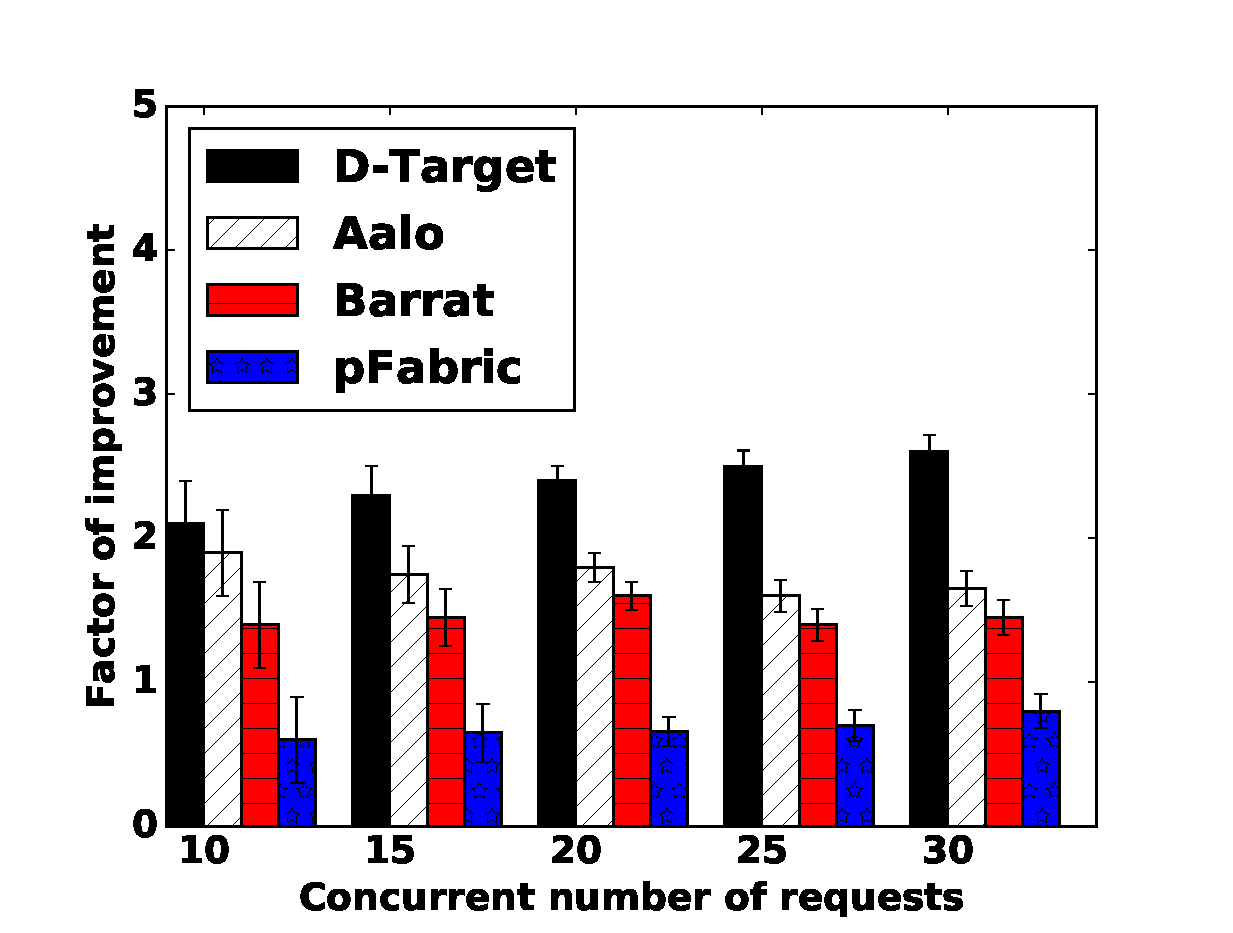
\includegraphics[width=0.33\textwidth]{picture/model/alpha.eps}}
\caption{Fluid model and ns-2 simulation comparison}
\label{fluid-model-fig}
\end{figure*}


\subsubsection{FDRC Fluid model}

To understand the behavior of FDRC, we build fluid model according to \cite{DCTCPAnalysis} and \cite{TCPfluid}.
Assume N flows transfer to the same receiver node through the bottleneck link whose capacity is C, the propagation delay
is pd and FDRC fluid model is:

\begin{align}
&\frac{d\alpha_i}{dt}=\frac{g}{R(t)}(p(t-R^*)-\alpha_i(t)) \label{model_alpha} \\
&\widehat{p}(t)=1_{\widehat{q}(t)>1}  \label{model_mark} \\
&\frac{dq}{dt}= \sum_{i=1}^N{\frac{w_i(t)}{R(t)}}-C \label{model_queue}  \\
&\frac{dw_i}{dt}=\frac{1-\alpha_i(t)\times d_{i}(t)}{R(t)}-\frac{w_i(t) \times \alpha_i(t)\times d_i(t)}{R(t)}p(t-R^*)  \label{model_window}
\end{align}

Equation (\ref{model_alpha})  and equation (\ref{model_mark})model the marking process of the switch.
Equation (\ref{model_queue}) models the queue and
Equation (\ref{model_window}) describes the congestion window of FDRC.



To verify our model, we start two long flows (f1.time\_start=0, f2.time\_start=0.5s). $DMAX=1,DMIN=0.5$ and the threshold: 
$threshold\_tight=0.3, threshold\_lax=0.6$. 
For flows whose duration time are less than 0.3 will have a largest value of deadline factor and
for flows whose duration time are larger than 0.6 will have smallest factor. 
Others' factors will drop with time goes by.
We use FDRC model to predict congestion window, $\alpha$ and queue. Then we compare the result with ns-2 simulation. 


Fig.\ref{fluid-model-fig}(a) depicts congestion window. We can observe that at first only flow1 starts, so flow1 occupies the total link bandwidth. Then at t=0.5, flow2 starts. 
As at t=0.5, flow2's factor is larger than flow1's, so flow2 has a larger congestion window. 
Then at t=1.1 they have the same value of congestion function factor.
Fig.\ref{fluid-model-fig}(b) shows queue size and Fig.\ref{fluid-model-fig}(c) depicts $\alpha$.  We can see that both Fluid model's queue length and $\alpha$
match quite well with the simulation result.

\subsubsection{Parameters selection}

In FDRC protocol, four global parameters should be set . Time threshold can be set according to application demand.
For example, in data center, flows may have deadline ranging from tight to lax, so threshold\_tight can be set
as tight deadline and threshold\_lax can be set as lax deadline.
In this part we will analyze how to set DMIN and DMAX.

At first, we get the fixed point of fluid model ($w_i$,$\alpha_i$,q)=($\frac{1}{d_i}$-1,1,$\sum_{i=1}^N \frac{1}{d_i}-N-C\times pd$).
The fixed point means all packets are all marked and senders have fixed congestion window. 
In reality, queue can not be too large, because a large queue size can result to a long queue delay. 
We assume in FDRC system, queue size should be shorter than
K+N, so we have:


\begin{equation}
\label{queuelength}
\sum_{i=1}^N \frac{1}{d_i}-N-C\times pd \le K+N
\end{equation}

As the factor d ranges between DMIN and DMAX, so for the scenery, flows' factor have the value of DMIN:
  
\begin{equation}
\label{DMAXvalue}
N \times \frac{1}{DMIN}-N-C\times pd \le K+N
\end{equation}

DMIN $\ge \frac{N}{2\times N +C \times pd +K}$. From (\ref{ca}), we know the congestion window function $f<1$, when $\alpha \times d$ achieves 1,$d<1$,
so DMAX and DMIN should be smaller than 1. DMIN and DMAX should satisfy:

\begin{equation}
\label{DMAXDMIN}
\frac{N}{2\times N +C \times pd +K} \le DMIN < DMAX \le1
\end{equation}

According to (\ref{DMAXDMIN}), we can conclude value of DMIN and DMAX can not be too small. 
Because small value of DMIN can make queue long, as a result flows will have
large queue delay and long latency.

\section {Evaluation} \label{evaluation}

In this section, we test the performance of FDRC under ns-2 simulation and small testbed.
We first solve the motivation problem that is proposed in the motivation section.
Then, we compare deadline miss between different protocols and our simulation result shows the percentage of deadline missing is only 1/5 of DCTCP.
After that,we verify the performance of flow completion time, we observe FDRC reduces about 50\% FCT than DCTCP.
At last, we evaluate FDRC in our small data center testbed.

\subsection{motivation resolved}

In this section, we first solve the problem that is proposed at section \ref{motivation}.  
For FDRC, we set $threshold_{lax}$=30ms and $threshold_{tight}$=10ms. 
DMAX = 0.5 and DMIN = 0.1. Fig.\ref{spineleaf--motivation-fig} shows the result. 
We can see, FDRC has less percentage of flows missing deadline than D2TCP
and flow completion time is shorter than L2DCT. 

The reason for this is that FDRC uses flow duration time as its rate control factor.
As for FDRC, $threshold_{lax}$=30ms and $threshold_{tight}$=10ms, so flows whose time constraints ranging from 10ms to 30ms,
will have larger average bandwidth than others.  For those emergency flows will have larger bandwidth than the lax ones, so less flows will miss deadline.
As flows have highest priority at first, then drops with time goes by, so short flows will have larger average bandwidth
than long-lived flows, as a result, the average flow completion time will reduce.


\begin{figure*}[!htb]
\centering
\subfloat[percentage of flows missing deadline]{
\label{spine-dc-data2-1}
\includegraphics[width=0.33\textwidth]{picture/evaluation/spineleaf/miss_deadline.eps}}
\subfloat[average flow completion time]{
\label{spine-dc-data2-5}
\includegraphics[width=0.33\textwidth]{picture/evaluation/spineleaf/fct2.eps}}
\subfloat[background traffic bandwidth]{
\label{spine-dc-data2-30}
\includegraphics[width=0.33\textwidth]{picture/evaluation/spineleaf/bandwidth.eps}}
\caption{motivation example: compare FDRC's performance with DCTCP, D2TCP and L2DCT}
\label{spineleaf--motivation-fig}
\end{figure*}


\subsection{At Scale Simulation In Spine-Leaf Data Center Topology}

To demonstrate FDRC's performance with real data center traffic and complex data center topology,
 we construct the spine\-leaf data topology in ns-2  \cite{ns2}. The topology is shown as Fig. \ref{DataCenterspineleaf-fig}.
In our simulation, there are 144 servers in total and 9 leaf switches connecting with 4 spine switches.
The end to end round trip latency across the spine switch (4 hops) is 14.6us and the end to end trip latency across the leaf switch (2 hops) is ~13.3us. 
Among the time, 10us is cost at the end server, this simulates the computation time of the servers. 
All the protocol of  experiment parameters we set are just the same as \cite{pFabric}.
\begin{figure}[b]
\centering
\includegraphics [width=0.8\columnwidth] {picture/evaluation/spineleaf/spineleaf.eps}
\caption{The spine-leaf Data Center topology}
\label{DataCenterspineleaf-fig}
\end{figure}


\emph{Benchmark workload}. We use two types of real data center workloads: 
web search workload and data mining workload\cite{DCTCP}\cite{pFabric}. 
For web search workload, 70\% flows are smaller than 1MB and more than 50\% of flows are between 100KB and 1MB. 
For data mining workload, more than 80\% flows are smaller than 10KB and more than 90\% bytes are from the 4\% large flows ($>1MB$).
In our simulation, different load means different rate of flows arrivals.
As today's datacenter network are often oversubscribed \cite{CloudMirror}, so in our experiments, 
we vary the oversubscription factor x  that is between the leaf switch and the spine switch to simulate this.

\emph{Performance metrics}. For deadline-constrained flows, we choose the percentage of flows missing deadline as the metrics to judge the performance of different algorithms.
We compare FDRC with the state-of-art deadline-aware congestion control algorithm LPD-e \cite{LPD},D2TCP \cite{D2TCP} and the deadline-agnostic protocol DCTCP \cite{DCTCP}.
For traffic that are deadline-agnostic, we consider average flow completion time and compare FDRC with pFabric \cite{pFabric}, DCTCP\cite{DCTCP} and L2DCT\cite{L2DCT}. 

\emph{Parameter selection}. Four important parameters are needed in FDRC. 
As in data center network, flows always have deadline constrains ranging from 10ms to 30ms \cite{D3}, 
so we choose $threshold_{lax}$=30ms and $threshold_{tight}$=10ms.
The factor boundary DMAX and DMIN can be set according to (\ref{DMAXDMIN}).
In our simulation, DMAX is 0.5 and DMIN is 0.1.




\subsubsection{Deadline miss comparison}\label{evaluation_deadline}

In data center, delay-sensitive business such as web search should transfer the 
computation results to client within some milliseconds, otherwise user experience will be affected. 
In this section, we test the performance of FDRC when traffic are delay-sensitive. 
In our experiment, we set \emph{Uniform} distribution deadline to flows to present users' expectation.
Flows arrive across a Poisson Process. 
Flow's source and destination are random chosen.
We also evaluate LPD-e, DCTCP and D2TCP  and compare them with FDRC.
Varying the oversubscription factor x and repeat each group of experiment 100 times,
then Fig. \ref{miss-spine-web-fig} shows the result. 



\begin{figure*}[!htb]
\centering
\subfloat[x=1]{
\label{spine-dc-web-1}
\includegraphics[width=0.25\textwidth]{picture/evaluation/spineleaf/miss_deadline_1.eps}}
\subfloat[x=4]{
\label{spine-dc-web--5}
\includegraphics[width=0.25\textwidth]{picture/evaluation/spineleaf/miss_deadline_3.eps}}
\subfloat[x=7]{
\label{spine-dc-web-10}
\includegraphics[width=0.25\textwidth]{picture/evaluation/spineleaf/miss_deadline_7.eps}}
\subfloat[x=10]{
\label{spine-dc-web-10}
\includegraphics[width=0.25\textwidth]{picture/evaluation/spineleaf/miss_deadline_10.eps}}
\caption{Deadline miss comparison between FDRC, LPD-e, D2TCP and DCTCP under web search workload. Flows' deadline have uniform distribution between 10ms and 30ms }
\label{miss-spine-web-fig}
\end{figure*}

We can see overall, FDRC performs better than D2TCP and DCTCP.  On average, FDRC reduces about 5X  percentage of flows missing deadline than DCTCP and reduce about 2X 
than D2TCP. The reason for its advantage is that FDRC has two threshold $threshold_{lax}$ (30ms) and $threshold_{tight}$ (10ms), when flow duration time is shorter than
$threshold_{tight}$, flow has the largest value of congestion window factor, so it can have large value of congestion window, thus rate. However, FDRC sometimes performs worse than LPD-e, this is because 
LPD-e adjusts congestion window using explicit deadline set by user, while FDRC is an implicit and indirect method. Although FDRC performs a little worse than
LPD-e (about 0.5\% more missing deadline), we regard FDRC as a better choice, because sometimes accurate deadline may be not easily known beforehand .

Specially, FDRC performs even well for the heavy congestion link condition. As Fig. \ref{miss-spine-web-fig}(a) shown, when the oversubscription factor x=1, FDRC is only 20\% better than D2TCP and when the factor 
x=10, Fig. \ref{miss-spine-web-fig}(d) shows it performs about 5X times better than D2TCP. The reason for this is that FDRC's follows the principle of more load, more differentiation \cite{LPD}.
The result is more or less the same for data mining workload just as Fig. \ref{miss-spine-data-fig} shows.
Note the reason for percentage of flow missing for data mining workload is a little larger than web search is that data mining traffic includes large flows ($>10MB$) which can easily miss deadline.


\begin{figure*}[!htb]
\centering
\subfloat[x=1]{
\label{spine-dc-data-1}
\includegraphics[width=0.25\textwidth]{picture/evaluation/spineleaf/miss_deadline_4.eps}}
\subfloat[x=4]{
\label{spine-dc-data--5}
\includegraphics[width=0.25\textwidth]{picture/evaluation/spineleaf/miss_deadline_6.eps}}
\subfloat[x=7]{
\label{spine-dc-data-10}
\includegraphics[width=0.25\textwidth]{picture/evaluation/spineleaf/miss_deadline_8.eps}}
\subfloat[x=10]{
\label{spine-dc-data-10}
\includegraphics[width=0.25\textwidth]{picture/evaluation/spineleaf/miss_deadline_9.eps}}
\caption{Deadline missing comparison between FDRC and LPD, D2TCP, DCTCP under data mining workload.  Flows' deadline have uniform distribution between 10ms and 30ms }
\label{miss-spine-data-fig}
\end{figure*}



\begin{figure*}[!htb]
\centering
\subfloat[tight deadline(10ms)]{
\label{spine-dc-data2-1}
\includegraphics[width=0.33\textwidth]{picture/evaluation/spineleaf/miss_deadline_tcp_tight.eps}}
\subfloat[mild deadline(20ms)]{
\label{spine-dc-data2-5}
\includegraphics[width=0.33\textwidth]{picture/evaluation/spineleaf/miss_deadline_tcp_mild.eps}}
\subfloat[lax deadline(30ms)]{
\label{spine-dc-data2-30}
\includegraphics[width=0.33\textwidth]{picture/evaluation/spineleaf/miss_deadline_tcp_lax.eps}}
\caption{Web Search workload of deadline missing comparison between FDRC and D2TCP, DCTCP. Note, in this experiment, deadline has exponential distribution and only half of the flows have deadline. }
\label{miss-spine-search-2-fig}
\end{figure*}



In data center network, not all flows are latency-constraint, some flows are background flows. In this experiment, we divide the web
search load traffic into two groups. The number of flows in each group is the same. 
For the first group, all flows have deadline which are exponential distribution.
The second group flows are background flows which are deadline-agnostic. 
We use three kind deadline:
tight (10ms), mild (20ms) and lax (30ms) \cite{D3} in our simulation. 
All flows arrive across a Poisson Process. The source and destination server are random chosen. Fig. \ref{miss-spine-search-2-fig} shows
the result. We can see that  FDRC as well as D2TCP works better than DCTCP and FDRC performs better than D2TCP in most cases. 
We observe that FDRC only improves about 20\%-30\% over D2TCP, while in the previous experiment, it improves 2X. The reason for
this is that, in this experiment, only half of the flows have deadline, FDRC treats the two group fair, but D2TCP let the first group flow have large congestion window.


 \begin{figure*}[t]
\centering
\subfloat[Average FCT]{
\label{spine-dc-search-5}
\includegraphics[width=0.33\textwidth]{picture/evaluation/spineleaf/FCT_SEARCH_average.eps}}
\subfloat[(500KB,+$\infty$) ]{
\label{spine-dc-search-5-large}
\includegraphics[width=0.33\textwidth]{picture/evaluation/spineleaf/FCT_SEARCH_large.eps}}
\subfloat[(0,100KB)]{
\label{spine-dc-search-5-small}
\includegraphics[width=0.33\textwidth]{picture/evaluation/spineleaf/FCT_SEARCH_small.eps}}
\caption{Web Search workload, comparison of average flow completion time between FDRC ,DCTCP, L2DCT and pFabric. Fig. (a) is the result of total flow. Fig. (b) shows the average of large flows($>500KB$) and 
Fig. (c) depicts the small ones}
\label{fct-spine-search-5-fig}
\end{figure*}

\begin{figure*}[t]
\centering
\subfloat[Average FCT]{
\label{spine-dc-data-5}
\includegraphics[width=0.33\textwidth]{picture/evaluation/spineleaf/FCT_DATA_average.eps}}
\subfloat[(500KB,+$\infty$) ]{
\label{spine-dc-data-5-large}
\includegraphics[width=0.33\textwidth]{picture/evaluation/spineleaf/FCT_DATA_large.eps}}
\subfloat[(0,100KB)]{
\label{spine-dc-data-5-small}
\includegraphics[width=0.33\textwidth]{picture/evaluation/spineleaf/FCT_DATA_small.eps}}
\caption{Data Mining workload,  comparison of average flow completion time between FDRC, DCTCP, L2DCT and pFabric. Fig. (a) is the result of total flow. Fig. (b) shows the average of large flows($>500KB$) and 
Fig. (c) depicts the small ones}
\label{fct-spine-data-5-fig}
\end{figure*}



\begin{figure*}[t]
\centering
\subfloat[Average FCT]{
\label{spine-dc-data-factor}
\includegraphics[width=0.33\textwidth]{picture/evaluation/spineleaf/fct.eps}}
\subfloat[(500KB,+$\infty$) ]{
\label{spine-dc-data-factor-large}
\includegraphics[width=0.33\textwidth]{picture/evaluation/spineleaf/large_fct.eps}}
\subfloat[(0,100KB)]{
\label{spine-dc-data-factor-small}
\includegraphics[width=0.33\textwidth]{picture/evaluation/spineleaf/small_fct.eps}}
\caption{Web Search workload, overall normalized average FCT for FDRC ,DCTCP and pFabric when we varying the oversubscription factor from 5 to 30.  Note that DCTCP does not appear in Fig.(c) as its value is larger than the plot range}
\label{fct-spine-fct-factor-fig}
\end{figure*}



\begin{figure}[b]
\centering
\includegraphics [width=0.8\columnwidth] {picture/evaluation/Realtest/testbed.eps}
\caption{The small scale data center testbed}
\label{testbed-fig}
\end{figure}

\begin{figure*}[!htb]
\centering
\subfloat[bandwidth]{
\label{testbed-rate}
\includegraphics[width=0.25\textwidth]{picture/evaluation/Realtest/rate.eps}}
\subfloat[queue]{
\label{testbed-queue}
\includegraphics[width=0.25\textwidth]{picture/evaluation/Realtest/realqueue.eps}}
\subfloat[deadline miss]{
\label{testbed-miss}
\includegraphics[width=0.25\textwidth]{picture/evaluation/Realtest/miss_deadline_.eps}}
\subfloat[FCT]{
\label{testbed-fct}
\includegraphics[width=0.25\textwidth]{picture/evaluation/Realtest/fct_.eps}}
\caption{Performance of FDRC under small testbed }
\label{tesbed-fig}
\end{figure*}


\subsubsection{Flow completion time comparison}\label{evaluation_fct}

For the whole fabric network,  optimal algorithm for minimizing average FCT is 
equivalent to the NP-hard sum multi-coloring problem \cite{COLOR}, but  when scheduling over a single link is the Shortest Remaining Processing Time (SRPT) 
policy which always schedules the flow that has the least work remaining. 
FDRC reduces flow completion time by letting those short flows have higher priority throughout their transfer life, which approximates SRPT schema.

We compare the performance between FDRC and DCTCP, L2DCT, pFabric. Fig. \ref{fct-spine-search-5-fig} depicts the flow completion time for web search traffic. From Fig. \ref{fct-spine-search-5-fig}(a), 
we can see that FDRC performs about 10\% better than L2DCT, but 20\% worse than the
nearly optimal state-of-art protocol pFabric \cite{pFabric}. To see some detail of the experiment, we divide the traffic into large and small and show their respect FCT. 
From Fig. \ref{fct-spine-search-5-fig}(b) we observe the large flows' average completion time is about 40ms, which is about 30\%-40\% larger than pFabric.
Fig. \ref{fct-spine-search-5-fig}(c) shows for those small flow, FDRC only lags about 5\% to pFabric. Fig. \ref{fct-spine-data-5-fig} shows the experiment result for data mining traffic.
As many traffic flow in data mining work load is less than 10KB, so the average completion time for data mining traffic is shorter than the web search environment.

We vary the oversubscription factor from 5 to 40 to test the performance of FDRC.
Fig. \ref{fct-spine-fct-factor-fig} shows the experiment result. From Fig. \ref{fct-spine-fct-factor-fig}(a), we can see that comparing with DCTCP, FDRC reduces
about 50\% completion time.  As FDRC also follows the principle "more load, more differentiation" \cite{LPD}, its performance can be guaranteed when congestion load is heavy. 
That's can explain why its performance improves more for the large oversubscription comparing with the small value.







\iffalse
\subsection{FDRC deep dive} \label{evaluation_deep}
In this section we dig deep into FDRC design in a series of targeted simulations. In our simulation, we construct the topology that 10 sender nodes connect with the receiver node through the 
router and all link capacity is 1Gbps. 


\subsubsection{application throughput}

In this section, we compare the application throughput between different protocol. In our experiment, 
2 senders send long-live background flows to the receiver and the other 8 senders send flows with
uniform distribution deadline between 10ms and 30ms. We define application throughput that the link utilization for flows which do not miss deadline. 


Fig. \ref{app-rate}(a) shows the result for data mining workload 
and Fig. \ref{app-rate}(b) shows the result for web search workload. 
We can see FDRC's application throughput is higher than both DCTCP and D2TCP.
 This is because FDRC has smaller percentage of flow missing than
DCTCP and D2TCP.

\begin{figure}[t]
\centering
\subfloat[Data Mining]{
\label{apprate-data}
\includegraphics[width=0.25\textwidth]{picture/evaluation/spineleaf/appliction_throughput_data.eps}}
\subfloat[Web Search]{
\label{apprate-websearch}
\includegraphics[width=0.25\textwidth]{picture/evaluation/spineleaf/appliction_throughput_search.eps}}
\caption{Fig. (a) shows the application rate for the data mining workload. Fig.(b) shows the application rate for web search workload}
\label{app-rate}
\end{figure}



The performance achieved by FDRC depends on the weights assigned to flows. 
The theoretical of  DMIN and DMAX has been 
analyzed at the pervious section. 
In this section, we evaluate the impact of varying DMAX and DMIN.
 According to (\ref{DMAXDMIN}),
 DMIN and DMAX can be set between 0.02 and 1.
In our simulation, we choose 1 sender to send background flow.

Fig. \ref{bound-fig}(a) and Fig. \ref{bound-fig}(b) show the impact of varying 
DMAX on the AFCT of short flows and the throughput of long-lived flows when the offered load is 0.5.
Observe that increasing DMAX can reduce the AFCT as well as the throughput of long flows.
This happens because increasing DMAX makes short flows aggressive time long.
 Since long flows back off significantly even for small $\alpha$, this reduces their throughput. 
Then, we vary DMIN. We can see that the AFCT of short flows and the throughput of long flow decreases 
when DMIN is increased as shown in Fig. \ref{bound-fig}(c) and Fig. \ref{bound-fig}(d). 
 This happens because increasing  DMIN can make the short flows more aggressive, thus reducing average flow completion time.
In our simulation , we set DMAX to 0.5 and DMIN to 0.1 to achieve a compromise between the performance of short and long flows.



\begin{figure*}[!htb]
\centering
\subfloat[DMIN=0.1]{
\label{spine-dc-data-1}
\includegraphics[width=0.25\textwidth]{picture/evaluation/parameter/max_fct.eps}}
\subfloat[DMIN=0.1]{
\label{spine-dc-data--5}
\includegraphics[width=0.25\textwidth]{picture/evaluation/parameter/max_throughput.eps}}
\subfloat[DMAX=0.9]{
\label{spine-dc-data-10}
\includegraphics[width=0.25\textwidth]{picture/evaluation/parameter/min_fct.eps}}
\subfloat[DMAX=0.9]{
\label{spine-dc-data-10}
\includegraphics[width=0.25\textwidth]{picture/evaluation/parameter/min_throughput.eps}}
\caption{impact of varying DMAX and DMIN on the AFCT of short flows and the throughput performance of long-lived flows. }
\label{bound-fig}
\end{figure*}
\fi

\subsection{small testbed evaluation} \label{evaluation_testbed}


To test the performance of FDRC under a real environment.
Based on DCTCP, we implement  D2TCP and LPD, L2DCT in Linux kernel 3.2.61.
We use the linux serve as switch which runs FreeBSD 9.1 along with DummyNet \cite{dummynet} \cite{MPTCP}  to construct a two-way bottleneck link,
so that packets can be forwarded and marked at line speed. Due to our limited hardware, we can only set up a small tree-based scale topology of 3 switches with 6 servers just
as Fig. \ref{testbed-fig} shown.




\subsubsection{bandwidth}

FDRC flows can have higher priority when they start and their priority will drop with time goes by.
In our testbed experiment, we set DMAX=0.5 and DMIN =0.1. The time threshold threshold\_{lax}=200ms, threshold\_{tight}=100ms.
K=40KB at the switch server.
We then start 4 flows, flow1 is from S1,starts at t=0s. flow2 from S2 and starts at t=0.3s. 
flow3 is from S3 and starts at t=0.4s. flow4 is from S3 and starts at t=0.5. All flows' destination are server R.


Fig. \ref{testbed-fig}(a) shows the result. We can see all flows will have largest bandwidth when start and begin to slow with time goes by.
Then at last, as all flows have the same priority, they share the link bandwidth. Fig. \ref{testbed-fig}(b) shows the queue length on server L1, we can see FDRC
can keep the queue at low and steady level.

\subsubsection{deadline miss comparison}

In this section we test the performance when there are delay-sensitive flows in data center.
In our experiment, firstly, each server $S_{i}$ first builds up a tcp connection with the random server. Each connection lasts T min. During the T min,
server $S_{i}$ will send small query flows to receiver. After T min, server $S_{i}$ will choose another random server and repeat the process.
We repeat the process 100 times and each group T= 5 minutes. 
We set DMAX=0.5 , DMIN =0.1 and the time threshold threshold\_{lax}=200ms, threshold\_{tight}=100ms, varying flow size,
then Fig. \ref{tesbed-fig}(c) shows the result.

We can observe FDRC performs better than DCTCP and D2TCP. It reduces about half the number of flow deadline missing than DCTCP and 
30\% less than D2TCP. But FDRC's performance is about 5\% worse than LPD.
The experiment result is almost the same as our simulation .
 
\subsubsection{flow completion time comparison}

In this section we test FDRC's performance on reducing flow completion time. In our experiment, firstly, each server $S_{i}$ first builds up a tcp connection with the random server.
 Each connection lasts T min. During the T min, the server random sends
 short flows to receiver.  After T min, server $S_{i}$ will choose another random server and repeat the process. We repeat the process 100 times and each group T= 5 minutes, then
Fig. \ref{tesbed-fig}(d) shows the result.

We can see that FDRC performs about 20\% better than DCTCP, about 10\% better than L2DCT and about 5\% worse than LPD. 
 



\section{conclusion} \label{conclusion}

In this paper, we use flow duration time to compute correction function factor.
We advocate this suitable, because by setting threshold, those urgent flows will get more bandwidth than the background flows, 
thus they can finish transferring before their time constraints. Based on this, we propose FDRC and model FDRC.
Then we test the performance of FDRC under ns-2 and linux kernel. Our experiments show FDRC
performs  30\% than D2TCP and L2DCT on average.


Although FDRC performs well under both simulation and small testbed. 
it requires rigorous analysis on stability and convergence properties,
we will study this in the near future.



\section{Acknowledgement}
This work is supported by the National High Technology Research and Development Program of China (863 Program) No. 2015AA015603, No. 2015AA016105
and the National Natural Science Foundation of China (Grant No. 61402253). 


\bibliographystyle{abbrv}
\bibliography{ATC}




% that's all folks
\end{document}


